\bookchapter{Why Rust for Robots}\label{ch:rust1}

\section*{Explanation}
Until now this book used Python: it is quick to write, has all the machine-learning libraries, and is the best language for experiments. The \emph{competition} robot, however, runs a program that must react every few milliseconds, for a whole match, without crashing, on a small computer inside the robot. For such programs our team uses \textbf{Rust}, and the tools that we use to look into the robot (the debugging client that shows sensor values and what the robot is thinking) are being rewritten in Rust as well, from Java and Node.js. This part of the book teaches you enough Rust to read and extend that code. You only need the Python of Part~\ref{part:python}.

\section*{What kind of language is Rust?}
Python is \textbf{interpreted}: a program (the interpreter) reads your text and carries it out line by line, at run time. Rust is \textbf{compiled}: a program called the \textbf{compiler} (\verb!rustc!, usually started through the build tool \verb!cargo!) translates your whole program once, \emph{before} it runs, into machine code for the processor. The result is a single file that the processor executes directly, with no interpreter and no Python installation on the robot. Because the compiler sees the whole program in advance it can also \emph{check} a lot: types, missing cases, and, specially in Rust, how memory is used.
\begin{center}
\begin{tikzpicture}[>={Stealth[length=2.5mm]},bx/.style={draw,thick,rounded corners=2pt,minimum width=2.6cm,minimum height=0.9cm,font=\footnotesize,align=center}]
 \node[bx,fill=blue!8] (py) at (0,1.2) {\texttt{prog.py}};
 \node[bx,fill=yellow!20] (it) at (3.6,1.2) {interpreter\\ (\texttt{python3})};
 \node[bx,fill=green!10] (r1) at (7.2,1.2) {result};
 \draw[->,thick] (py)--(it); \draw[->,thick] (it)--(r1);
 \node[font=\scriptsize,gray,anchor=west,text width=3.8cm] at (8.8,1.2) {runs at once, errors show up while running};
 \node[bx,fill=orange!12] (rs) at (0,-0.4) {\texttt{main.rs}};
 \node[bx,fill=yellow!20] (co) at (3.6,-0.4) {compiler\\ (\texttt{rustc})};
 \node[bx,fill=gray!15] (bin) at (7.2,-0.4) {executable\\ (machine code)};
 \draw[->,thick] (rs)--(co); \draw[->,thick] (co)--(bin);
 \node[font=\scriptsize,gray,anchor=west,text width=3.8cm] at (8.8,-0.4) {many errors are found \emph{before} the first run};
\end{tikzpicture}
\captionof{figure}{Interpreted and compiled: the compiler is a strict reader that works before the program exists as a running process.}
\end{center}

\section*{Reason 1: speed that you can plan with}
A simulation step of a damped spring (a model of a robot leg) is a few multiplications. We ran the same loop in Python and in Rust (the Rust program is in Chapter~\ref{ch:rust2}) on the computer used to write this book:
\begin{center}
\renewcommand{\arraystretch}{1.2}
\begin{tabular}{lrr}
\textbf{program} & \textbf{time per step} & \textbf{relative}\\ \hline
Python 3.13 & 229\,ns & $26\times$\\
Rust, release build & 8.9\,ns & $1\times$\\
\end{tabular}
\end{center}
($5$ million steps in $1143$\,ms in Python; $50$ million steps in $445$\,ms in Rust.) Python is slow here because each simple operation on a number is a call into the interpreter: look up the variables, check the types, create a new number object. Rust compiles the operations into a few processor instructions on plain numbers. In Python we avoid the problem by moving the loop into NumPy (Chapter~\ref{ch:py8}), which is itself written in a compiled language, but that works only for operations on whole arrays. The control loop of a robot is full of \emph{decisions} that depend on the previous step; in Rust you can write them straightforwardly and still be fast.
\begin{keyidea}[Debug and release builds]
The numbers above are for the \textbf{release} build (\verb!cargo build --release!), which optimises. The default \textbf{debug} build compiles quickly and is easy to debug, but is much slower: in a second test, ten passes of a small iterator chain over $10$ million numbers took $1828$\,ms in a debug build, $217$\,ms in a release build, and a single pass in Python took $725$\,ms. Always measure speed with \verb!--release!, and never judge Rust by its debug build.
\end{keyidea}
\begin{center}
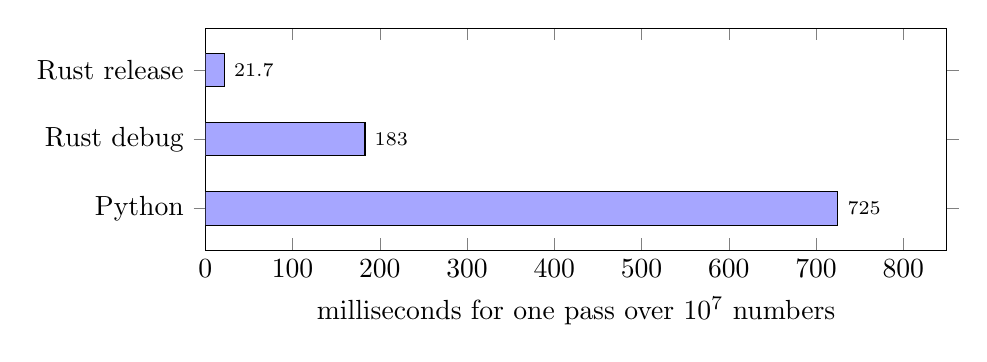
\begin{tikzpicture}
\begin{axis}[xbar,width=11cm,height=4.4cm,bar width=12pt,xmin=0,xmax=850,
 xlabel={milliseconds for one pass over $10^7$ numbers},
 symbolic y coords={Rust release,Rust debug,Python},ytick=data,
 nodes near coords,nodes near coords align={horizontal},every node near coord/.append style={font=\scriptsize},
 y dir=reverse,enlarge y limits=0.3]
 \addplot[fill=blue!35] coordinates {(21.7,Rust release) (183,Rust debug) (725,Python)};
\end{axis}
\end{tikzpicture}
\captionof{figure}{Measured time for the same small calculation (filter, square, sum); the Rust numbers are one tenth of ten passes.}
\end{center}

\section*{Reason 2: no pauses and no surprises in time}
Python and Java free memory with a \textbf{garbage collector}: now and then the runtime stops to look for objects that are no longer used. The pause may be short, but it comes at a time you do not choose, and a robot that is balancing or kicking cannot wait. Rust has no garbage collector. It decides at \emph{compile time} when each piece of memory is no longer needed and frees it at exactly that place in the program (Chapter~\ref{ch:rust3}). The time a loop needs is therefore much more predictable. (The operating system still does other things, so Rust alone does not make a program \emph{real-time}; see the discussion of jitter in Chapter~\ref{ch:ros6}.)

\section*{Reason 3: the compiler finds bugs before the robot does}
Older systems languages like C and C++ are fast as well, but they let the programmer make mistakes with memory that crash the program or, worse, produce wrong values silently:
\begin{itemize}[nosep]
\item using memory after it was freed (\emph{use after free});
\item reading past the end of an array (\emph{buffer overflow});
\item two threads changing the same data at the same time (\emph{data race});
\item using a variable that was never given a value.
\end{itemize}
Rust makes these mistakes \textbf{compile errors}. The price is that the compiler is strict and sometimes rejects a program that you believe is fine; learning to work with the compiler is the main effort of learning Rust (Chapters~\ref{ch:rust3} and~\ref{ch:rust6}). The reward is a sentence you will hear Rust programmers say: ``if it compiles, it usually works''. That sentence is not a proof (a wrong formula compiles perfectly well), but it is true often enough to be valuable on a robot that you cannot attach a debugger to in the middle of a match.
Other helpful properties: types are checked (a distance in metres is not silently added to a count), a value that may be missing is a different type from one that is always there (no ``\verb!None! has no attribute'' surprise at run time, Chapter~\ref{ch:rust4}), and every case of a choice must be handled.

\section*{Reason 4: one file to deploy}
A Rust program is one executable file. To run it on the robot you copy the file; there is no Python version to match, no virtual environment (Chapter~\ref{ch:linux4}), no pip. The same source can be compiled on your laptop for the processor of the robot (\textbf{cross-compilation}, Chapter~\ref{ch:rust10}), and the tools that the team uses (the debug client) can be delivered to every student laptop in the same way.

\section*{Where Python is still the better choice}
Rust is not better at everything, and the honest comparison is part of the lesson.
\begin{center}
\renewcommand{\arraystretch}{1.25}
\begin{tabular}{p{4.3cm}p{4.6cm}p{4.6cm}}
\textbf{} & \textbf{Python} & \textbf{Rust}\\ \hline
First working version & minutes & longer, the compiler asks questions\\
Experiments, plots, notebooks & excellent & not made for it\\
Machine learning & the standard (Part~\ref{part:ai}) & mostly runs models, rarely trains them\\
Speed of the code you write & slow for loops & fast\\
Behaviour in a long run & errors appear at run time & many errors found by the compiler\\
Deploying to the robot & Python + packages & one file\\
\end{tabular}
\end{center}
Our team therefore uses both: Python for training, data analysis and video analysis (Part~\ref{part:bonus}), Rust for the program that runs on the robot and for the tools that connect to it. Very often a feature is first tried in Python and then rewritten in Rust once it is clear what it should do.

\section*{The system that we are going to build}
The Rust chapters of this book lead to the following picture, the same one the team uses.
\begin{center}
\begin{tikzpicture}[>={Stealth[length=2.5mm]},bx/.style={draw,thick,rounded corners=2pt,minimum width=2.8cm,minimum height=1.0cm,font=\footnotesize,align=center}]
 \node[bx,fill=green!12] (cam) at (0,2) {sensors,\\ camera};
 \node[bx,fill=blue!10] (ros) at (4,2) {ROS~2\\ (sensor topics)};
 \node[bx,fill=orange!15] (rob) at (8.2,2) {robot program\\ (Rust)};
 \node[bx,fill=yellow!20] (cli) at (8.2,-0.4) {debug client\\ (Rust, TUI)};
 \node[bx,fill=gray!15] (log) at (4,-0.4) {log files\\ (protobuf)};
 \draw[->,thick] (cam)--(ros); \draw[->,thick] (ros)--(rob);
 \draw[<->,thick] (rob)--node[right,font=\scriptsize,align=left]{UDP +\\ protobuf} (cli);
 \draw[->,thick] (cli)--(log);
 \node[font=\scriptsize,gray] at (4,0.6) {Chapters \ref{ch:rust7}, \ref{ch:rust8}};
 \node[font=\scriptsize,gray] at (9.9,0.9) {};
\end{tikzpicture}
\captionof{figure}{The robot program reads sensor data from ROS~2, and talks to the debugging client over UDP with messages encoded as protobuf (Chapters~\ref{ch:rust7} and~\ref{ch:rust8}); the client is a terminal application (Chapter~\ref{ch:rust9}) that can also write the data to log files. Chapter~\ref{ch:rust11} shows how Rust meets ROS~2.}
\end{center}

\begin{aibox}[Learn Rust with the compiler]
The error messages of the Rust compiler are famously good: they point at the exact place, explain what is wrong and often suggest the fix. Read them from the top. Do not try to understand the whole message at once; the first lines usually say all you need.
\end{aibox}

\section*{Practice problems}
\begin{enumerate}[label=\textbf{\thechapter.\arabic*}]
  \item Explain in two sentences the difference between an interpreter and a compiler. Which one needs to be installed on the robot to run a finished program?
  \item In the loop benchmark, Python needed $229$\,ns per step and Rust $8.9$\,ns. How many steps can each language do in a control period of $2$\,ms if the whole period were used for this loop?
  \item A simulation needs $3\cdot10^{9}$ steps. How long does it take with the times of the benchmark (in seconds and minutes)?
  \item In the second benchmark a debug build needed $1828$\,ms and a release build $217$\,ms for the same work. By which factor is the release build faster? Why do we still use debug builds while developing?
  \item Name the four kinds of memory error listed in this chapter, and give for each one an example of what could happen on a robot.
  \item A garbage collector pauses a program for $30$\,ms every few seconds. The robot's balance loop runs at $200$\,Hz. How many control steps are lost during one pause? Which consequence could that have?
  \item Say for each task which language you would choose and why: (a) plotting the learning curve of a network, (b) the program that reads the IMU and sends motor commands $200$ times per second, (c) a one-time script that renames $500$ video files, (d) the debug client that shows live data from the robot on a student laptop.
  \item ``If it compiles, it works.'' Give an example of a mistake that the Rust compiler \emph{cannot} find. What do you need besides the compiler to find it?
  \item What is cross-compilation and why is it useful if the robot's computer is slower than your laptop and has a different kind of processor?
  \item[\textbf{\thechapter.10}$\star$] A colleague proposes to rewrite the whole video-analysis project (Part~\ref{part:bonus}) in Rust ``because it is faster''. Write down the arguments for and against in five sentences, using the table of this chapter, and give your recommendation. Which measurement would you make first?
\end{enumerate}
